\newif\ifalone
\alonefalse
\newif\iftalk
\talkfalse

\ifalone
\documentclass{article}
\usepackage{graphicx}
\usepackage{natbib}
\usepackage{amsfonts}
\usepackage{amssymb}
\usepackage{amsthm}
\usepackage{bm}
\usepackage{Sweave}
\usepackage{lscape}
\usepackage{makeidx}
\usepackage{color}
\title{Multi-response models}

\author{Jarrod Hadfield (\texttt{j.hadfield@ed.ac.uk})}
\begin{document}
\maketitle
\else
\chapter{Multi-response models}
\label{chap5}
\fi



So far we have only fitted models to a single response variable.  Multi-response models are not that widely used, except perhaps in quantitative genetics, and deserve wider use. They allow some of the assumptions of single response models to be relaxed and can be an effective way of dealing with missing data problems. 

\section{Relaxing the univariate assumptions of causality}

Imagine we knew how much money 200 people had spent on their holiday and on their car in each of four years, and we want to know whether a relationship exists between the two.  A simple correlation would be one possibility, but then how do we control for the repeated measures? An often used solution to this problem is to choose one variable as the response (lets say the amount spent on a car) and have the other variable as a fixed covariate (the amount spent on a holiday).  The choice is essentially arbitrary, highlighting the belief that any relationship between the two types of spending maybe in part due to unmeasured variables, rather than being completely causal.\\

In practice does this matter? Lets imagine there was only one unmeasured variable: disposable income. There are repeatable differences between individuals in their disposable income, but also some variation within individuals across the four years.  Likewise, people vary in what proportion of their disposable income they are willing to spend on a holiday versus a car, but this also changes from year to year.  We can simulate some toy data to get a feel for the issues: 

\begin{Schunk}
\begin{Sinput}
> id<-gl(200,4)                  # 200 people recorded four times                      
> av_wealth<-rlnorm(200, 0, 1)               
> ac_wealth<-av_wealth[id]+rlnorm(800, 0, 1) 
> # expected disposable incomes + some year to year variation
> 
> av_ratio<-rbeta(200,10,10)                 
> ac_ratio<-rbeta(800, 2*(av_ratio[id]), 2*(1-av_ratio[id])) 
> # expected proportion spent on car + some year to year variation
> 
> y.car<-(ac_wealth*ac_ratio)^0.25     # disposable income * proportion spent on car
> y.hol<-(ac_wealth*(1-ac_ratio))^0.25 # disposable income * proportion spent on holiday                              
> Spending<-data.frame(y.hol=y.hol, y.car=y.car, id=id)
\end{Sinput}
\end{Schunk}

A simple regression suggests the two types of spending are negatively related but the association is weak with the $R^{2}=$ 0.005.

\begin{Schunk}
\begin{Sinput}
> summary(lm(y.car ~ y.hol, data = Spending))
\end{Sinput}
\begin{Soutput}
Call:
lm(formula = y.car ~ y.hol, data = Spending)

Residuals:
     Min       1Q   Median       3Q      Max 
-0.84047 -0.19337 -0.01766  0.18888  1.27426 

Coefficients:
            Estimate Std. Error t value Pr(>|t|)    
(Intercept)  1.07739    0.03750  28.732   <2e-16 ***
y.hol       -0.06937    0.03429  -2.023   0.0434 *  
---
Signif. codes:  0 '***' 0.001 '**' 0.01 '*' 0.05 '.' 0.1 ' ' 1 

Residual standard error: 0.3059 on 798 degrees of freedom
Multiple R-squared: 0.005104,	Adjusted R-squared: 0.003858 
F-statistic: 4.094 on 1 and 798 DF,  p-value: 0.04336 
\end{Soutput}
\end{Schunk}

With \texttt{id} added as a random term to deal with the the repeated measures, a similar conclusion is reached although the estimate is more negative:

\iftalk
\else
\fi

\begin{Schunk}
\begin{Sinput}
> m5a.1 <- MCMCglmm(y.car ~ y.hol, random = ~id, data = Spending, 
+     verbose = FALSE)
> summary(m5a.1$Sol[, "y.hol"])
\end{Sinput}
\begin{Soutput}
Iterations = 3001:12991
Thinning interval = 10 
Number of chains = 1 
Sample size per chain = 1000 

1. Empirical mean and standard deviation for each variable,
   plus standard error of the mean:

          Mean             SD       Naive SE Time-series SE 
     -0.185720       0.035786       0.001132       0.001058 

2. Quantiles for each variable:

   2.5%     25%     50%     75%   97.5% 
-0.2505 -0.2106 -0.1881 -0.1620 -0.1111 
\end{Soutput}
\end{Schunk}

 We may be inclined to stop there, but lets proceed with a multi-response model of the problem. The two responses are passed as a matrix using \texttt{cbind()}, and the rows of this matrix are indexed by the reserved variable {\color{red} \texttt{units}}, and the columns by the reserved variable \texttt{\color{blue} \texttt{trait}}.\\ 

It is useful to think of a new data frame where the response variables have been stacked column-wise and the other predictors duplicated accordingly. Below is the original data frame on the left (\texttt{Spending}) and the stacked data frame on the right:\\  

\begin{displaymath}
\begin{array}{cc}
\begin{array}{cccc}
&{\color{blue} \texttt{y.hol}}&{\color{blue} \texttt{y.car}}&\texttt{id}\\
{\color{red} \texttt{1}}&\texttt{1.060184}&\texttt{0.781681}&\texttt{1}\\
{\color{red} \texttt{2}}&\texttt{0.943428}&\texttt{1.328910}&\texttt{1}\\
\vdots&\vdots&\vdots\\
{\color{red} \texttt{800}}&\texttt{0.952169}&\texttt{1.038891}&\texttt{200}\\
\end{array}&
\Longrightarrow
\begin{array}{ccccc}
&\texttt{y}&{\color{blue} \texttt{trait}}&\texttt{id}&{\color{red} \texttt{units}}\\
1&\texttt{1.060184}&{\color{blue} \texttt{y.hol}}&\texttt{1}&{\color{red} \texttt{1}}\\
2&\texttt{0.943428}&{\color{blue} \texttt{y.hol}}&\texttt{1}&{\color{red} \texttt{2}}\\
\vdots&\vdots&\vdots&\vdots\\
800&\texttt{0.952169}&{\color{blue} \texttt{y.hol}}&\texttt{200}&{\color{red} \texttt{800}}\\
801&\texttt{0.781681}&{\color{blue} \texttt{y.car}}&\texttt{1}&{\color{red} \texttt{1}}\\
802&\texttt{1.328910}&{\color{blue} \texttt{y.car}}&\texttt{1}&{\color{red} \texttt{2}}\\
\vdots&\vdots&\vdots&\vdots\\
1600&\texttt{1.038891}&{\color{blue} \texttt{y.car}}&\texttt{200}&{\color{red} \texttt{800}}\\
\end{array}
\end{array}
\end{displaymath}

From this we can see that fitting a multi-response model is a direct extension to how we fitted models with categorical random interactions \ref{chap3}:

\begin{Schunk}
\begin{Sinput}
> m5a.2 <- MCMCglmm(cbind(y.hol, y.car) ~ trait - 1, random = ~us(trait):id, 
+     rcov = ~us(trait):units, data = Spending, family = c("gaussian", 
+         "gaussian"), verbose = FALSE)
\end{Sinput}
\end{Schunk}

We have fitted the fixed effect \texttt{trait} so that the two types of spending can have different intercepts. I usually suppress the intercept (\texttt{-1}) for these types of models so the second coefficient is not the difference between the intercept for the first level of \texttt{trait} (\texttt{y.hol}) and the second level (\texttt{y.car}) but the actual trait specific intercepts. In other words the design matrix for the fixed effects has the form:

\begin{displaymath}
\begin{array}{rl}
\left[
\begin{array}{cc}
\texttt{trait[1]=="y.hol"}&\texttt{trait[1]=="y.car"}\\
\texttt{trait[2]=="y.hol"}&\texttt{trait[2]=="y.car"}\\
\vdots&\vdots\\
\texttt{trait[800]=="y.hol"}&\texttt{trait[800]=="y.car"}\\
\texttt{trait[801]=="y.hol"}&\texttt{trait[801]=="y.car"}\\
\texttt{trait[802]=="y.hol"}&\texttt{trait[802]=="y.car"}\\
\vdots&\vdots\\
\texttt{trait[1600]=="y.hol"}&\texttt{trait[1600]=="y.car"}\\
\end{array}
\right]
=&
\left[
\begin{array}{cc}
1&0\\
1&0\\
\vdots&\vdots\\
1&0\\
0&1\\
0&1\\
\vdots&\vdots\\
0&1\\
\end{array}
\right]\\
\end{array}
\end{displaymath}

A $2\times2$ covariance matrix is estimated for the random term where the diagonal elements are the variance in consistent individual effects for each type of spending. The off-diagonal is the covariance between these effects which if positive suggests that people that consistently spend more on their holidays consistently spend more on their cars. A $2\times2$ residual covariance matrix is also fitted. In Section \ref{heter-sec}  we fitted heterogeneous error models using \texttt{idh():units} which made sense in this case because each level of \texttt{unit} was specific to a particular datum and so any covariances could not be estimated.   In multi-response models this is not the case because both traits have often been measured on the same observational unit and so the covariance can be measured. In the context of this example a positive covariance would indicate that in those years an individual spent a lot on their car they also spent a lot on their holiday.\\

A univariate regression is defined as the covariance between the response and the predictor divided by the variance in the predictor. We can therefore estimate a regression coefficient for these two levels of random variation, and compare them with the regression coefficient we obtained in the simpler model:
 
\begin{Schunk}
\begin{Sinput}
> id.regression <- m5a.2$VCV[, 2]/m5a.2$VCV[, 1]
> units.regression <- m5a.2$VCV[, 6]/m5a.2$VCV[, 5]
> plot(mcmc.list(m5a.1$Sol[, "y.hol"], id.regression, units.regression), 
+     density = FALSE)
\end{Sinput}
\end{Schunk}

The regression coefficients (see Figure \ref{asUV-fig})differ substantially at the within individual (green) and between individual (red) levels, and neither is entirely consistent with the regression coefficient from the univariate model (black). The process by which we generated the data gives rise to this phenomenon - large variation between individuals in their disposable income means that people who are able to spend a lot on their holiday can also afford to spend a lot on their holidays (hence a positive covariation between \texttt{id} effects). However, a person that spent a large proportion of their disposable income in a particular year on a holiday, must have less to spend that year on a car (hence a negative residual (within year) covariation). \\    



\iftalk
\else
\fi


\begin{figure}[!h]
\begin{center}
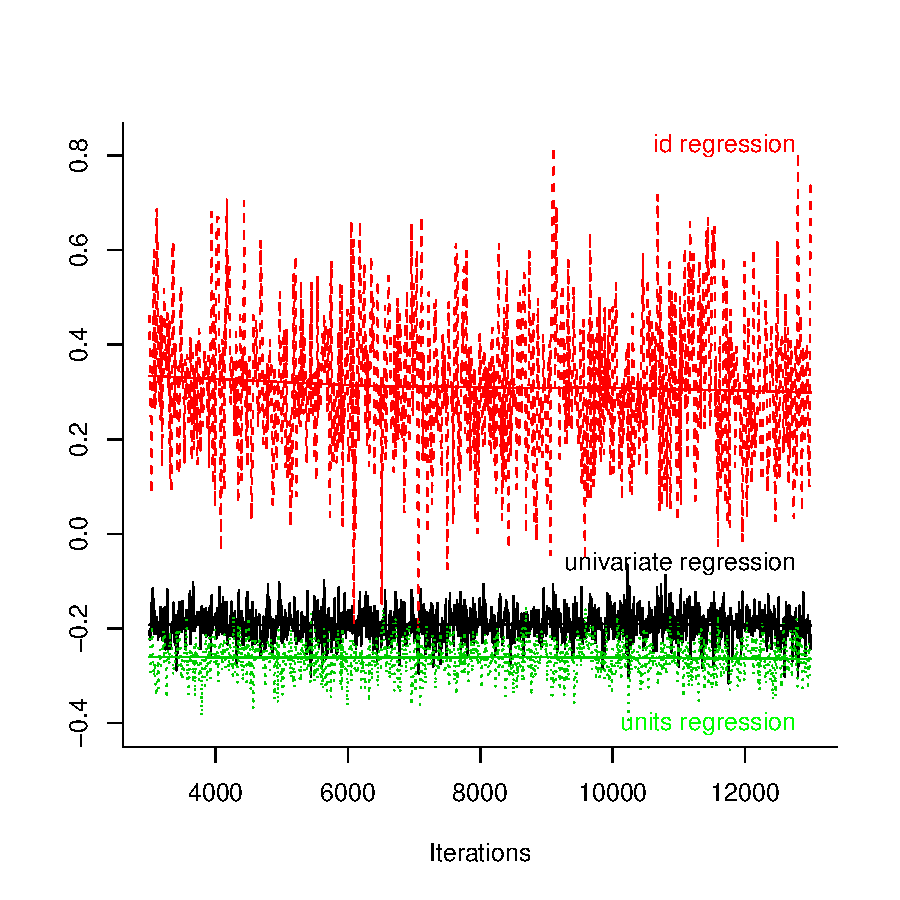
\includegraphics{Lecture5-011}
\end{center}
\caption{MCMC summary plot of the coefficient from a regression of car spending on holiday spending in black. The red and green traces are from a model where the regression coefficient is estimated at two levels: within an individual (green) and across individuals (red). The relationship between the two types of spending is in part mediating by a third unmeasured variable, disposable income.}
\label{asUV-fig}
\end{figure}

When fitting the simpler univariate model we make the assumption that the effect of spending money on a car directly effects how much you spend on a holiday. If this relationship was purely causal then all regression coefficients would have the same expectation, and the simpler model would be justified.\\

For example, we could set up a simpler model where two thirds of the variation in holiday expenditure is due to between individual differences, and holiday expenditure directly affects how much an individual will spend on their car (using a regression coefficient of -0.3). The variation in car expenditure not caused by holiday expenditure is also due to individual differences, but in this case they only explain a third of the variance.  

\begin{Schunk}
\begin{Sinput}
> Spending$y.hol2 <- rnorm(200, 0, sqrt(2))[Spending$id] + rnorm(800, 
+     0, sqrt(1))
> Spending$y.car2 <- Spending$y.hol2 * -0.3 + rnorm(200, 0, sqrt(1))[Spending$id] + 
+     rnorm(800, 0, sqrt(2))
\end{Sinput}
\end{Schunk}

We can fit the univariate and multivariate models to these data, and compare the regression coefficients as we did before. Figure \ref{MVvUV2-fig} shows that the regression coefficients are all very similar and a value of -0.3 has a reasonably high posterior probability. However, it should be noted that the posterior standard deviation is smaller in the simpler model because the more strict assumptions have allowed us to pool information across the two levels to get a more precise answer.   


\iftalk
\else
\fi
\begin{figure}[!h]
\begin{center}
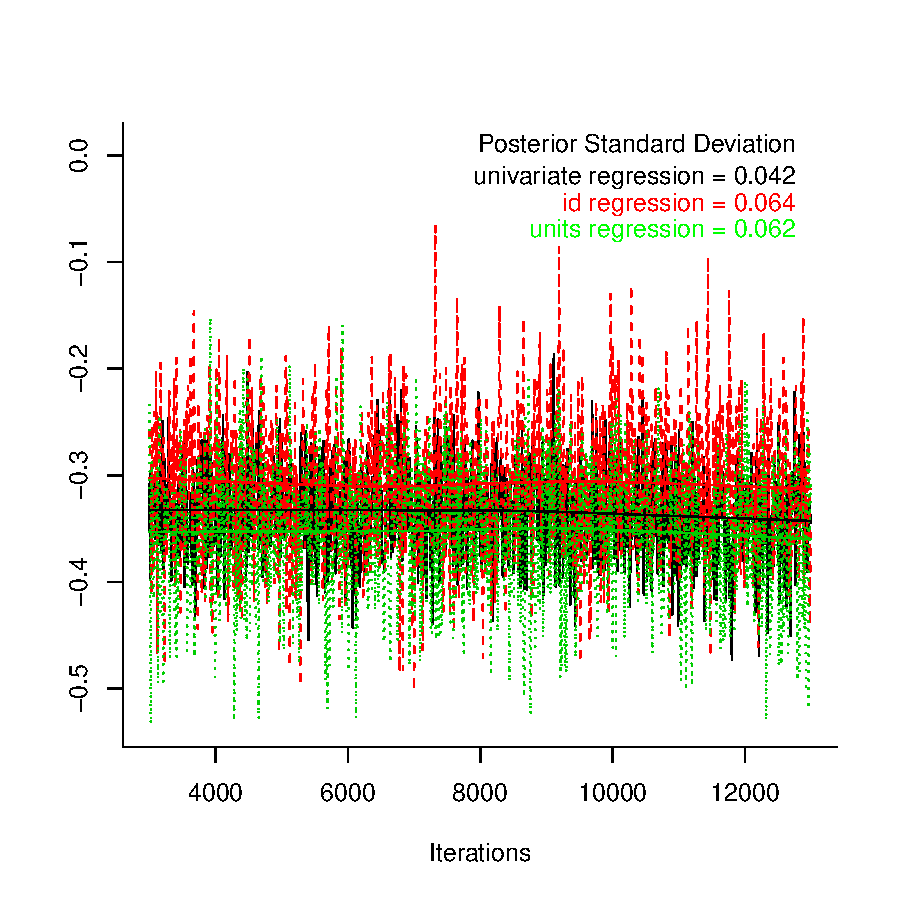
\includegraphics{Lecture5-016}
\end{center}
\caption{MCMC summary plot of the coefficient from a regression of car spending on holiday spending in black. The red and green traces are from a model where the regression coefficient is estimated at two levels: within an individual (green) and across individuals (red). In this model the relationship between the two types of spending is causal and the regression coefficients have the same expectation. However, the posterior standard deviation from the simple regression is smaller because information from the two different levels is pooled.}
\label{MVvUV2-fig}
\end{figure}

\section{Multinomial Models}

Multinomial models are difficult - both to fit and interpret.  This is particularly true when each unit of observation only has a single realisation from the multinomial. In these instances the data can be expressed as a single vector of factors, and the family argument can be specified as \texttt{categorical}.  To illustrate, using a very simple example, we'll use data collected on 666 Soay sheep from the island of Hirta in the St. Kilda archipelago \citep[][Table A2.5]{Clutton-Brock.2004}. 


\begin{Schunk}
\begin{Sinput}
> data(SShorns)
> head(SShorns)
\end{Sinput}
\begin{Soutput}
  id    horn    sex
1  1 scurred female
2  2 scurred female
3  3 scurred female
4  4 scurred female
5  5  polled female
6  6  polled female
\end{Soutput}
\end{Schunk}

The sex and horn morph were recorded for each individual, giving the contingency table:  

\begin{Schunk}
\begin{Sinput}
> Ctable <- table(SShorns$horn, SShorns$sex)
> Ctable
\end{Sinput}
\begin{Soutput}
          female male
  normal      83  352
  polled      65    0
  scurred     96   70
\end{Soutput}
\end{Schunk}

and we'll see if the frequencies of the three \texttt{horn} types differ, and if the trait is sex dependent. The usual way to do this would be to use a Chi square test, and to address the first question we could add the counts of the two sexes: 

\begin{Schunk}
\begin{Sinput}
> chisq.test(rowSums(Ctable))
\end{Sinput}
\begin{Soutput}
	Chi-squared test for given probabilities

data:  rowSums(Ctable) 
X-squared = 329.5225, df = 2, p-value < 2.2e-16
\end{Soutput}
\end{Schunk}

which strongly suggests the three morphs differ in frequency. We could then ask whether the frequencies differ by sex:

\begin{Schunk}
\begin{Sinput}
> chisq.test(Ctable)
\end{Sinput}
\begin{Soutput}
	Pearson's Chi-squared test

data:  Ctable 
X-squared = 202.2962, df = 2, p-value < 2.2e-16
\end{Soutput}
\end{Schunk}

which again they do, which is not that surprising since the trait is partly sex limited, with males not expressing the polled phenotype.\\

If there were only two horn types, polled and normal for example, then we could have considered transforming the data into the binary variable \emph{polled or not?} and analysing using a glm with sex as a predictor. In doing this we have reduced the dimension of the data from $J=2$ categories to a single ($J-1=1$) contrast. The motivation for the dimension reduction is obvious; if being a male increased the probability of expressing normal horns by 10\%, it must by necessity reduce the probability of expressing polled horn type by 10\%, because an individual cannot express both horn types  simultaneously.  The dimension reduction essentially constrains the probability of expressing either horn type to unity:\\

\begin{equation}
Pr(\texttt{horn[i]}=\textrm{normal})+Pr(\texttt{horn[i]}=\textrm{polled}) = 1
\end{equation}

These concepts can be directly translated into situations with more than two categories where the unit sum constraint has the general form:

\begin{equation}
\sum_{k=1}^{J}Pr(y_{i}=k)=1 
\end{equation}

 For binary data we designated one category to be the success (polled) and one category to be the failure (normal) which we will call the baseline category.  The latent variable in this case was the log-odds ratio  of succeeding versus failing:

\begin{equation}
 l_{i} = \textrm{log}\left(\frac{Pr(\texttt{horn[i]}=\textrm{polled})}{Pr(\texttt{horn[i]}=\textrm{normal})}\right) = \textrm{logit}\left(Pr(\texttt{horn[i]}=\textrm{polled})\right)
\end{equation}

With more than two categories we need to have $J-1$ latent variables, which in the original horn type example are:

\begin{equation}
l_{i,\textrm{polled}} = \textrm{log}\left(\frac{Pr(\texttt{horn[i]}=\textrm{polled})}{Pr(\texttt{horn[i]}=\textrm{normal})}\right)
\end{equation}

and 

\begin{equation}
l_{i,\textrm{scurred}} = \textrm{log}\left(\frac{Pr(\texttt{horn[i]}=\textrm{scurred})}{Pr(\texttt{horn[i]}=\textrm{normal})}\right)
\end{equation}


The two latent variables are indexed as \texttt{trait}, and the unit of observation ($i$) as \texttt{units}, as in multi-response models. As with binary models the residual variance is not identified, and can be set to any arbitrary value. For reasons that will become clearer later I like to work with the residual covariance matrix $\frac{1}{J}({\bf I}+{\bf J})$ where  ${\bf I}$ and ${\bf J}$ are $J-1$ dimensional identity and unit matrices, respectively.

To start we will try a simple model with an intercept:\\

\begin{Schunk}
\begin{Sinput}
> IJ <- (1/3) * (diag(2) + matrix(1, 2, 2))
> prior = list(R = list(V = IJ, fix = 1))
> m5c.1 <- MCMCglmm(horn ~ trait - 1, rcov = ~us(trait):units, 
+     prior = prior, data = SShorns, family = "categorical", verbose = FALSE)
\end{Sinput}
\end{Schunk}

The posterior distribution for the intercepts is shown in Figure \ref{MN1}, and the model clearly needs to be run for longer. However...\\


\begin{figure}[!h]
\begin{center}
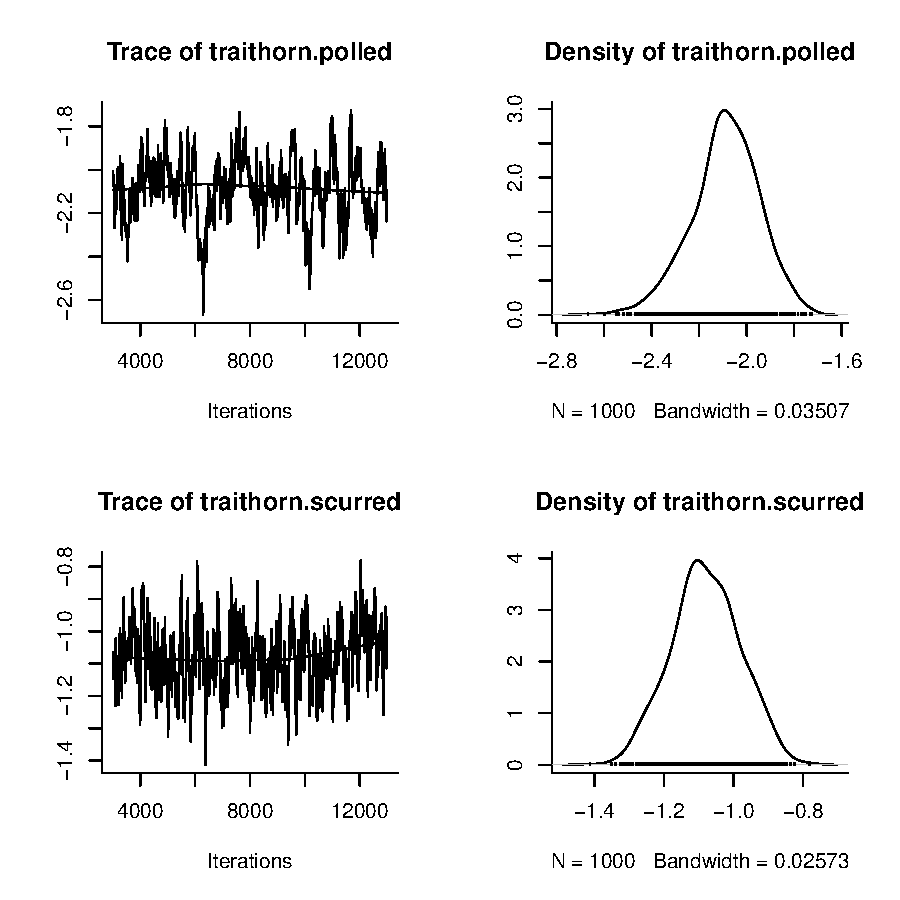
\includegraphics{Lecture5-024}
\end{center}
\caption{Posterior distribution of fixed effects from model \texttt{m5c.1}: a simple multinomial logit model with intercepts only}
\label{MN1}
\end{figure}



The problem can also be represented using the contrast matrix ${\bf \Delta}$ \citep{Bunch.1991}:

\begin{equation}
{\bm \Delta}=
\left[
\begin{array}{c c}
-1&-1\\
1&0\\
0&1\\
\end{array}
\right]
\end{equation}

where the rows correspond to the factor levels (\texttt{normal}, \texttt{polled} and \texttt{scurred}) and the columns to the two latent variables. For example column one corresponds to $l_{i,\textrm{polled}}$ which on the log scale is $Pr(\texttt{horn[i]}=\textrm{polled}) - Pr(\texttt{horn[i]}=\textrm{normal})$.\\

\begin{equation}
\textrm{exp}\left(({\bm \Delta}{\bm \Delta}^{'})^{-1}{\bm \Delta}{\bf l}_{i}\right) \propto E\left[\begin{array}{c} Pr(\texttt{horn[i]}=\textrm{normal})\\ Pr(\texttt{horn[i]}=\textrm{polled})\\ Pr(\texttt{horn[i]}=\textrm{scurred}) \end{array} \right]
\end{equation}

The residual and any random effect covariance matrices are for estimability purposes estimated on the $J-1$ space with  ${\bm V}={\bm \Delta}^{'}\tilde{\bf V}{\bm \Delta}$ where $\tilde{\bf V}$ is the covariance matrix estimated on the $J-1$ space. To illustrate, we will rescale the intercepts as if the residual covariance matrix was zero (see Sections and \label{pred-sec} \label{cat-sec}) and predict the expected probability for each horn type:

\begin{Schunk}
\begin{Sinput}
> Delta <- cbind(c(-1, 1, 0), c(-1, 0, 1))
> c2 <- (16 * sqrt(3)/(15 * pi))^2
> D <- ginv(Delta %*% t(Delta)) %*% Delta
> Int <- t(apply(m5c.1$Sol, 1, function(x) {
+     D %*% (x/sqrt(1 + c2 * diag(IJ)))
+ }))
> summary(mcmc(exp(Int)/rowSums(exp(Int))))
\end{Sinput}
\begin{Soutput}
Iterations = 1:1000
Thinning interval = 1 
Number of chains = 1 
Sample size per chain = 1000 

1. Empirical mean and standard deviation for each variable,
   plus standard error of the mean:

       Mean      SD  Naive SE Time-series SE
[1,] 0.6537 0.01923 0.0006082       0.001913
[2,] 0.1018 0.01179 0.0003727       0.001565
[3,] 0.2446 0.01676 0.0005301       0.001637

2. Quantiles for each variable:

       2.5%    25%    50%    75%  97.5%
var1 0.6136 0.6421 0.6543 0.6659 0.6916
var2 0.0800 0.0934 0.1010 0.1094 0.1266
var3 0.2126 0.2340 0.2442 0.2549 0.2784
\end{Soutput}
\end{Schunk}

which agrees well with those observed:

\begin{Schunk}
\begin{Sinput}
> prop.table(rowSums(Ctable))
\end{Sinput}
\begin{Soutput}
   normal    polled   scurred 
0.6531532 0.0975976 0.2492492 
\end{Soutput}
\end{Schunk}

To test for the effects of sex specific expression we can also fit a model with a sex effect:

\begin{Schunk}
\begin{Sinput}
> m5c.2 <- MCMCglmm(horn ~ trait + sex - 1, rcov = ~us(trait):units, 
+     data = SShorns, family = "categorical", prior = prior, verbose = FALSE)
\end{Sinput}
\end{Schunk}

In this case we have not interacted sex with trait, and so we are estimating the difference between the sexes in their expression of normal and polled+scurred jointly. The posterior distribution is plotted in Figure \ref{MN2} and clearly shows that males are more likely to express the normal horn phenotype than females.


\begin{figure}[!h]
\begin{center}
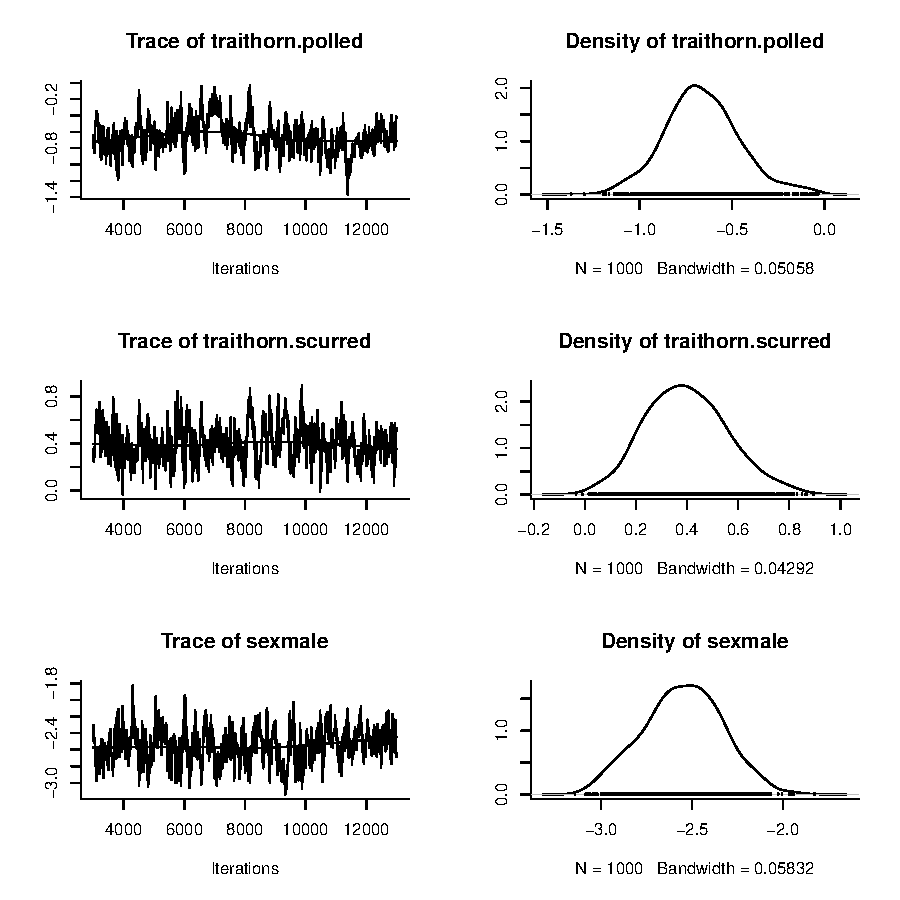
\includegraphics{Lecture5-029}
\end{center}
\caption{Posterior distribution of fixed effects from model \texttt{m5c.2} in which a main effect of sex was included}
\label{MN2}
\end{figure}

A more general model would be to fit estimate separate probabilities for each cell, but the contingency table indicates that one cell (polled males) has zero counts which will cause extreme separation problems. We could choose to have a better prior for the fixed effects, that is close to being flat for the two-way (i.e. polled vs scurred, normal vs.scurred \& polled vs. normal) marginal probabilities within each sex:

\begin{Schunk}
\begin{Sinput}
> prior$B = list(mu = rep(0, 4), V = kronecker(IJ, diag(2)) * (1.7 + 
+     pi^2/3))
> m5c.3 <- MCMCglmm(horn ~ at.level(sex, 1):trait + at.level(sex, 
+     2):trait - 1, rcov = ~us(trait):units, data = SShorns, family = "categorical", 
+     prior = prior, verbose = FALSE)
\end{Sinput}
\end{Schunk}

The female specific probabilities appear reasonable:

\begin{Schunk}
\begin{Sinput}
> Int <- t(apply(m5c.3$Sol[, 1:2], 1, function(x) {
+     D %*% (x/sqrt(1 + c2 * diag(IJ)))
+ }))
> summary(mcmc(exp(Int)/rowSums(exp(Int))))
\end{Sinput}
\begin{Soutput}
Iterations = 1:1000
Thinning interval = 1 
Number of chains = 1 
Sample size per chain = 1000 

1. Empirical mean and standard deviation for each variable,
   plus standard error of the mean:

       Mean      SD  Naive SE Time-series SE
[1,] 0.3484 0.03042 0.0009620       0.003264
[2,] 0.2634 0.02782 0.0008799       0.003189
[3,] 0.3882 0.03096 0.0009792       0.003607

2. Quantiles for each variable:

       2.5%    25%    50%    75%  97.5%
var1 0.2928 0.3275 0.3473 0.3684 0.4125
var2 0.2117 0.2444 0.2615 0.2836 0.3168
var3 0.3298 0.3669 0.3878 0.4097 0.4458
\end{Soutput}
\end{Schunk}

compared to the observed frequencies:

\begin{Schunk}
\begin{Sinput}
> prop.table(Ctable[, 1])
\end{Sinput}
\begin{Soutput}
   normal    polled   scurred 
0.3401639 0.2663934 0.3934426 
\end{Soutput}
\end{Schunk}

as do the male probabilities:

\begin{Schunk}
\begin{Sinput}
> Int <- t(apply(cbind(m5c.3$Sol[, 3:4]), 1, function(x) {
+     D %*% (x/sqrt(1 + c2 * diag(IJ)))
+ }))
> summary(mcmc(exp(Int)/rowSums(exp(Int))))
\end{Sinput}
\begin{Soutput}
Iterations = 1:1000
Thinning interval = 1 
Number of chains = 1 
Sample size per chain = 1000 

1. Empirical mean and standard deviation for each variable,
   plus standard error of the mean:

         Mean       SD  Naive SE Time-series SE
[1,] 0.826901 0.017160 0.0005427      0.0018916
[2,] 0.007024 0.004017 0.0001270      0.0004983
[3,] 0.166075 0.016442 0.0005199      0.0018214

2. Quantiles for each variable:

         2.5%      25%      50%     75%   97.5%
var1 0.793137 0.815633 0.827045 0.83895 0.85880
var2 0.002679 0.003802 0.005384 0.00986 0.01618
var3 0.136267 0.154557 0.166033 0.17673 0.19945
\end{Soutput}
\end{Schunk}

compared to the observed frequencies:

\begin{Schunk}
\begin{Sinput}
> prop.table(Ctable[, 2])
\end{Sinput}
\begin{Soutput}
   normal    polled   scurred 
0.8341232 0.0000000 0.1658768 
\end{Soutput}
\end{Schunk}


\section{Zero-inflated Models}

Each datum in a zero-inflated model is associated with two latent variables. The first latent variable is associated with the named distribution and the second latent variable is associated with zero inflation. I'll work through a zero-inflated Poisson (ZIP) model to make things clearer. As the name suggests, a ZIP distribution is a Poisson distribution with extra zero's. The observed zeros are modelled as a mixture distribution of zero's originating form the Poisson process and zero's arising through zero-inflation. It is the probability (on the logit scale) that a zero is from the zero-inflation process that we aim to model with the second latent variable. The likelihood has the form:

\begin{equation} 
\begin{array}{rl}
Pr(y | y=0) =& \texttt{plogis}(l_{2})+\texttt{plogis}(-l_{2})\ast \texttt{dpois}(0, \texttt{exp}(l_{1}))\\
Pr(y | y>0) =& \texttt{plogis}(-l_{2})\ast \texttt{dpois}(y, \texttt{exp}(l_{1}))\\
\end{array}
\end{equation}


{\bf pscl} fits zero-inflated models very well through the \texttt{zeroinfl} function, and I strongly recommend using it if you do not want to fit random effects. To illustrate the syntax for fitting ZIP models in MCMCglmm I will take one of their examples:   

\begin{Schunk}
\begin{Sinput}
> data("bioChemists", package = "pscl")
> head(bioChemists)
\end{Sinput}
\begin{Soutput}
  art   fem     mar kid5  phd ment
1   0   Men Married    0 2.52    7
2   0 Women  Single    0 2.05    6
3   0 Women  Single    0 3.75    6
4   0   Men Married    1 1.18    3
5   0 Women  Single    0 3.75   26
6   0 Women Married    2 3.59    2
\end{Soutput}
\end{Schunk}

\texttt{art} is the response variable - the number of papers published by a Ph.D student - and the remaining variables are to be fitted as fixed effects.  Naively, we may expect zero-inflation to be a problem given  30\% of the data are zeros, and based on the global mean we only expect around 18\%.

\begin{Schunk}
\begin{Sinput}
> table(bioChemists$art == 0)
\end{Sinput}
\begin{Soutput}
FALSE  TRUE 
  640   275 
\end{Soutput}
\begin{Sinput}
> ppois(0, mean(bioChemists$art))
\end{Sinput}
\begin{Soutput}
[1] 0.1839859
\end{Soutput}
\end{Schunk}

As with binary models we do not observe any residual variance for the zero-inflated process, and in addition the residual covariance between the zero-inflation and the Poisson process cannot be estimated because both processes cannot be observed in a single data point. To deal with this I've fixed the residual variance for the zero-inflation at 1, and the covariance is set to zero using the idh structure. Setting \texttt{V=diag(2)} and \texttt{nu=0.002}\footnote{Earlier versions of the CourseNotes had \texttt{nu=1.002}. In versions $<$2.05 the marginal prior of a variance associated with an \texttt{idh} structure was inverse-Wishart with $\texttt{nu}^{\ast}=\texttt{nu}-1$ where $\texttt{nu}^{\ast}$ is the marginal degree of belief. In versions $>=$2.05 I changed this so that $\texttt{nu}^{\ast}=\texttt{nu}$ as it was leading to confusion.} we have the inverse-gamma prior with \texttt{shape=scale=0.001} for the residual component of the Poisson process which captures over-dispersion:

\begin{Schunk}
\begin{Sinput}
> prior.m5d.1 = list(R = list(V = diag(2), nu = 0.002, fix = 2))
> m5d.1 <- MCMCglmm(art ~ trait - 1 + at.level(trait, 1):fem + 
+     at.level(trait, 1):mar + at.level(trait, 1):kid5 + at.level(trait, 
+     1):phd + at.level(trait, 1):ment, rcov = ~idh(trait):units, 
+     data = bioChemists, prior = prior.m5d.1, family = "zipoisson", 
+     verbose = FALSE)
\end{Sinput}
\end{Schunk}

As is often the case the parameters of the zero-inflation model mixes poorly (See Figure \ref{ZIP}) especially when compared to equivalent hurdle models (See Section \ref{Hurdle}). Poor mixing is often associated with distributions that may \emph{not} be zero-inflated but instead over-dispersed.\\  


\begin{figure}[!h]
\begin{center}
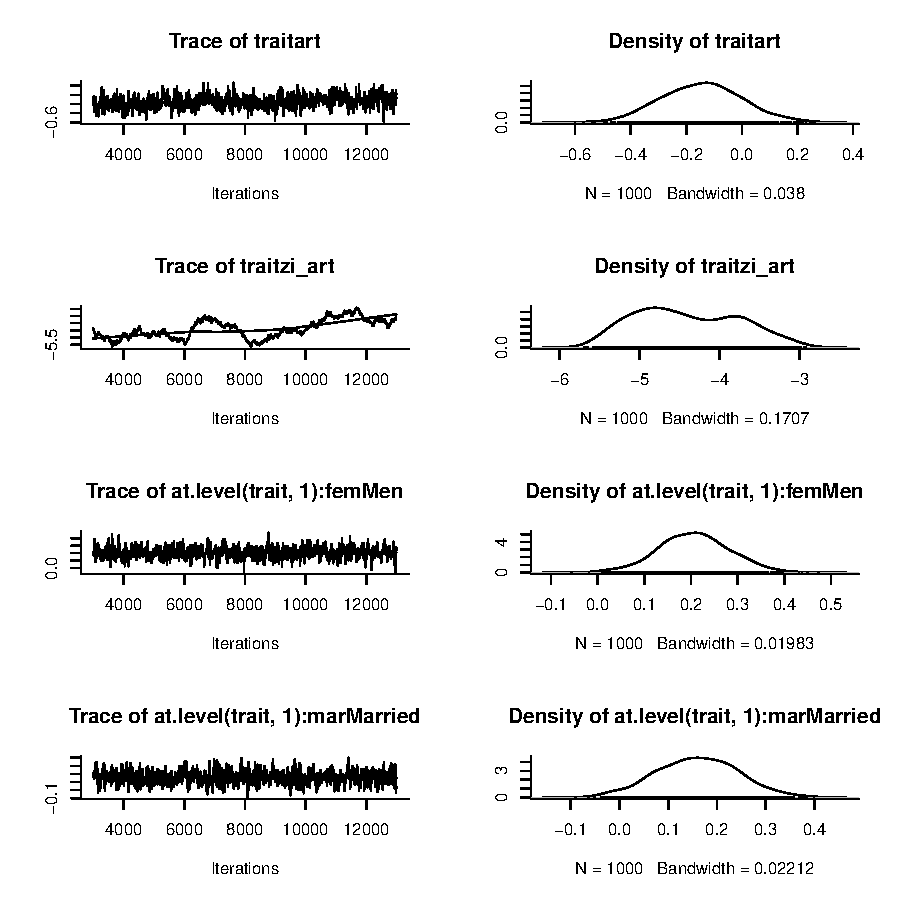
\includegraphics{Lecture5-039}
\end{center}
\caption{Posterior distribution of fixed effects from model \texttt{m5d.1} in which trait 1 (\texttt{art}) is the Poisson process and trait 2 (\texttt{zi.art}) is the zero-inflation.}
\label{ZIP}
\end{figure}

The model would have to be run for (much) longer to say something concrete about the level of zero-inflation but my guess would be it's not a big issue, given the probability is probably quite small:

\begin{Schunk}
\begin{Sinput}
> quantile(plogis(m5d.1$Sol[, 2]/sqrt(1 + c2)))
\end{Sinput}
\begin{Soutput}
          0%          25%          50%          75%         100% 
0.0008606214 0.0035960174 0.0056180399 0.0223208172 0.0603134988 
\end{Soutput}
\end{Schunk}

\subsection{Posterior predictive checks}

Another useful check is to fit the standard Poisson model and use posterior predictive checks to see how many zero's you would expect under the simple model:

\begin{Schunk}
\begin{Sinput}
> prior.m5d.2 = list(R = list(V = diag(1), nu = 0.002))
> m5d.2 <- MCMCglmm(art ~ fem + mar + kid5 + phd + ment, data = bioChemists, 
+     prior = prior.m5d.2, family = "poisson", saveX = TRUE, verbose = FALSE)
> nz <- 1:1000
> oz <- sum(bioChemists$art == 0)
> for (i in 1:1000) {
+     pred.l <- rnorm(915, (m5d.2$X %*% m5d.2$Sol[i, ])@x, sqrt(m5d.2$VCV[i]))
+     nz[i] <- sum(rpois(915, exp(pred.l)) == 0)
+ }
\end{Sinput}
\end{Schunk}

Figure \ref{PPZIP}  shows a histogram of the posterior predictive distribution of zero's from the model (\texttt{nz}) compared to the observed number of zeros (\texttt{oz}). The simpler model seems to be consistent with the data, suggesting that a ZIP model may not be required.


\begin{figure}[!h]
\begin{center}
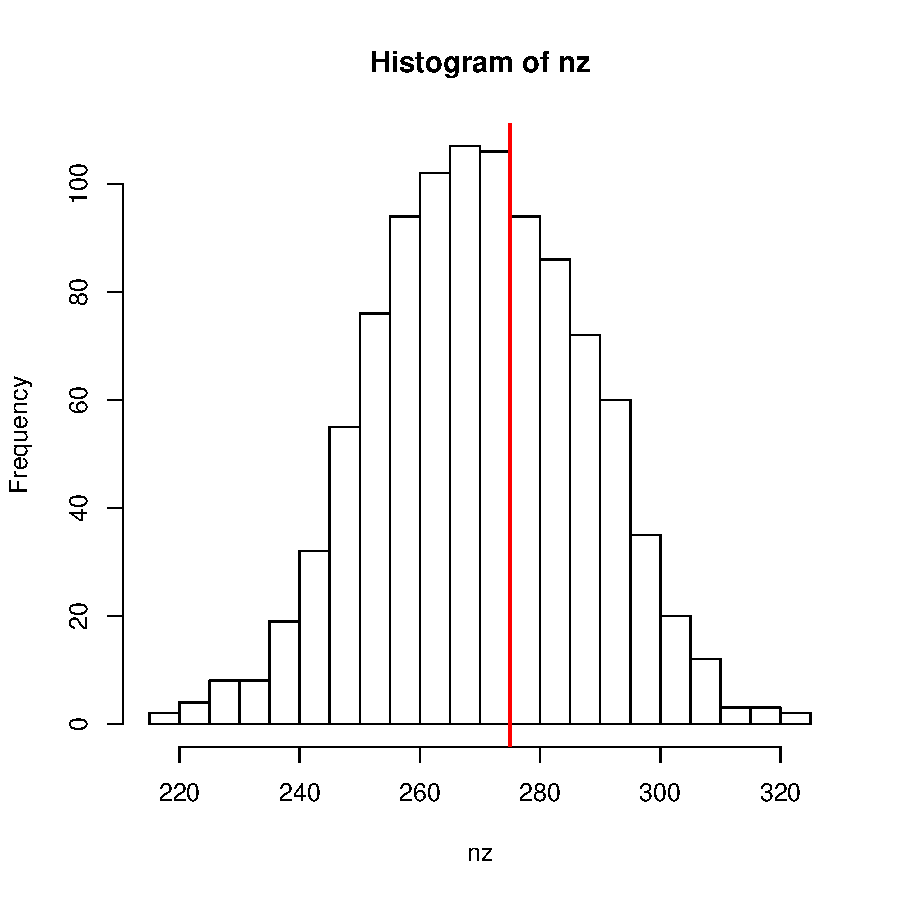
\includegraphics{Lecture5-043}
\end{center}
\caption{Posterior predictive distribution of zeros from model \texttt{m5d.2} with the observed number in red.}
\label{PPZIP}
\end{figure}

\section{Hurdle Models}
\label{Hurdle}

Hurdle models are very similar to zero-inflated models but they can be used to model zero-deflation as well as zero-inflation and seem to have much better mixing properties.  As in ZIP models each datum in the hurdle model is associated with two latent variables. However, whereas in a ZIP model the first latent variable is the mean parameter of a Poisson distribution the equivalent latent variable in the hurdle model is the mean parameter of a zero-truncated Possion distribution (i.e. a Poisson distribution without the zeros  observed). In addition the second latent variable in a ZIP model is the probability that an observed zero is due to zero-inflation rather than the Poisson process. In hurdle models the second latent variable is simply the probability (on the logit scale) that the response variable is zero or not. The likelihood is:

\begin{equation} 
\begin{array}{rl}
Pr(y | y=0) =& \texttt{plogis}(l_{2})\\
Pr(y | y>0) =& \texttt{plogis}(-l_{2})\ast \texttt{dpois}(y, \texttt{exp}(l_{1}))/(1-\texttt{ppois}(0, \texttt{exp}(l_{1})))\\
\end{array}
\end{equation}

 To illustrate, we will refit the ZIP model (\texttt{m5d.1}) as a hurdle-Poisson model.

\begin{Schunk}
\begin{Sinput}
> m5d.3 <- MCMCglmm(art ~ trait - 1 + at.level(trait, 1):fem + 
+     at.level(trait, 1):mar + at.level(trait, 1):kid5 + at.level(trait, 
+     1):phd + at.level(trait, 1):ment, rcov = ~idh(trait):units, 
+     data = bioChemists, prior = prior.m5d.1, family = "hupoisson", 
+     verbose = FALSE)
\end{Sinput}
\end{Schunk}

Plotting the Markov chain for the equivalent parameters that were plotted for the ZIP model shows that the mixing properties are much better (compare Figure \ref{ZIP} with Figure \ref{HU}).


\begin{figure}[!h]
\begin{center}
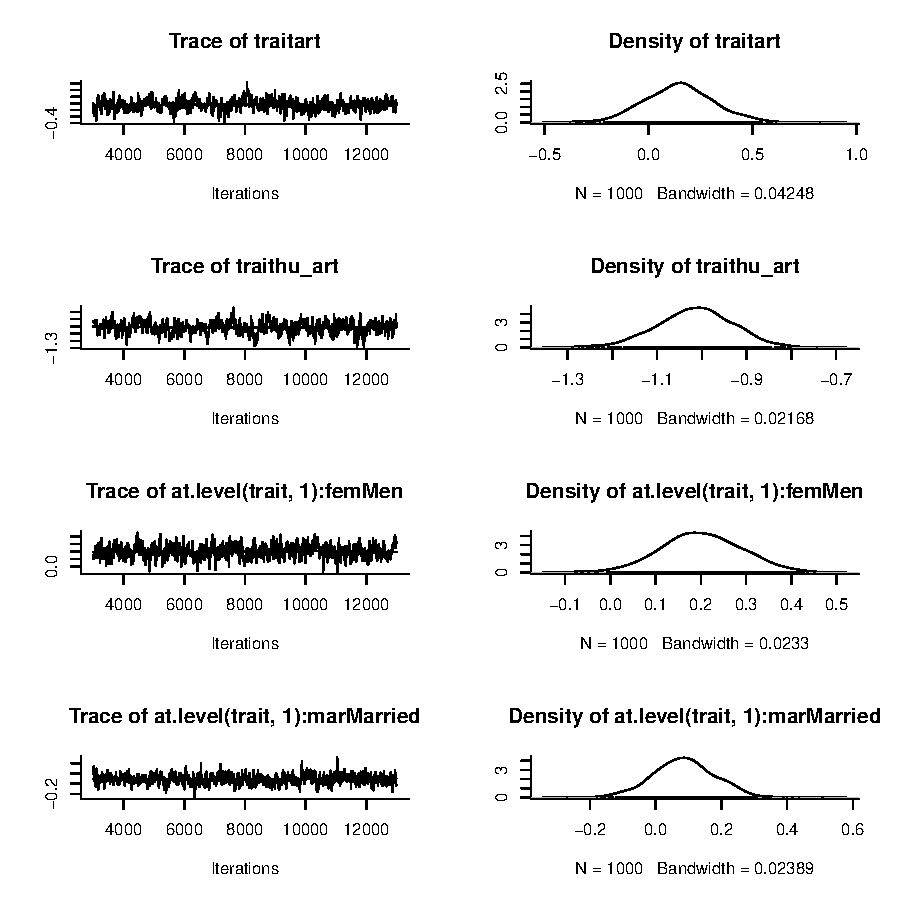
\includegraphics{Lecture5-046}
\end{center}
\caption{Posterior distribution of fixed effects from model \texttt{m5d.3} in which trait 1 (\texttt{art}) is the zero-truncated Poisson process and trait 2 (\texttt{hu.art}) is the binary trait zero or non-zero.}
\label{HU}
\end{figure}

The interpretation of the model is slightly different. Fitting just an intercept in the hurdle model implies that the proportion of zeros observed across different combinations of those fixed effects fitted for the Poisson process is constant. Our 95\% credible intervals for this proportion is (See section \ref{pred-sec}):

\begin{Schunk}
\begin{Sinput}
> c2 <- (16 * sqrt(3)/(15 * pi))^2
> HPDinterval(plogis(m5d.3$Sol[, 2]/sqrt(1 + c2)))
\end{Sinput}
\begin{Soutput}
         lower     upper
var1 0.2646899 0.3245956
attr(,"Probability")
[1] 0.95
\end{Soutput}
\end{Schunk}

and we can compare this to the predicted number of zero's from the Poisson process if it had not been zero-truncated:

\begin{Schunk}
\begin{Sinput}
> HPDinterval(ppois(0, exp(m5d.3$Sol[, 1] + 0.5 * m5d.3$VCV[, 1])))
\end{Sinput}
\begin{Soutput}
         lower     upper
var1 0.1514388 0.3775762
attr(,"Probability")
[1] 0.95
\end{Soutput}
\end{Schunk}

The credible intervals largely overlap, strongly suggesting a standard Poisson model would be adequate. However, our prediction for the number of zero's that would arise form a non-truncated Poisson process only involved the intercept term. This prediction therefore pertains to the number of articles published by single women with no young children who obtained their Ph.D's from departments scoring zero for prestige (\texttt{phd}) and whose mentors had published nothing in the previous 3 years.  Our equivalent prediction for men is a little lower 

\begin{Schunk}
\begin{Sinput}
> HPDinterval(ppois(0, exp(m5d.3$Sol[, 1] + m5d.3$Sol[, 3] + 0.5 * 
+     m5d.3$VCV[, 1])))
\end{Sinput}
\begin{Soutput}
         lower     upper
var1 0.0998876 0.2906499
attr(,"Probability")
[1] 0.95
\end{Soutput}
\end{Schunk}

suggesting that perhaps the number of zero's is greater than we expected for this group. However, this may just be a consequence of us fixing the proportion of zero's to be constant across these groups. We can relax this assumption by fitting a separate term for the proportion of zeros for men:

\begin{Schunk}
\begin{Sinput}
> m5d.4 <- MCMCglmm(art ~ trait - 1 + at.level(trait, 1:2):fem + 
+     at.level(trait, 1):mar + at.level(trait, 1):kid5 + at.level(trait, 
+     1):phd + at.level(trait, 1):ment, rcov = ~idh(trait):units, 
+     data = bioChemists, prior = prior.m5d.1, family = "hupoisson", 
+     verbose = FALSE)
\end{Sinput}
\end{Schunk}

which reveals that although this proportion is expected to be (slightly) smaller: 


\begin{Schunk}
\begin{Sinput}
> HPDinterval(plogis((m5d.4$Sol[, 2] + m5d.4$Sol[, 4])/sqrt(1 + 
+     c2)))
\end{Sinput}
\begin{Soutput}
         lower     upper
var1 0.2294218 0.3084297
attr(,"Probability")
[1] 0.95
\end{Soutput}
\end{Schunk}


the proportion of zeros expected for men is probably still less than what we expect from a non-truncated Poisson process for which the estimates have changed very little:

\begin{Schunk}
\begin{Sinput}
> HPDinterval(ppois(0, exp(m5d.4$Sol[, 1] + m5d.4$Sol[, 3] + 0.5 * 
+     m5d.4$VCV[, 1])))
\end{Sinput}
\begin{Soutput}
          lower     upper
var1 0.08358276 0.2462583
attr(,"Probability")
[1] 0.95
\end{Soutput}
\end{Schunk}


This highlights one of the disadvantages of hurdle models. If explanatory variables have been fitted that affect the expectation of the Poisson process than this implies that the proportion of zero's observed will also vary across these same explanatory variables, even in the absence of zero-inflation. It may then be necessary to fit an equally complicated model for both processes even though a single parameter would suffice in a ZIP model. However, in the absence of zero-inflation the intercept of the zero-inflation process in a ZIP model is $-\infty$ on the logit scale causing numerical and inferential problems. An alternative model are zero-altered models. 

\section{Zero-altered Models}
\label{ZAP}

Zero-altered Poisson (ZAP) models are identical to Poisson-hurdle models except a complementary log-log link is used instead of the logit link when modeling the proportion of zeros. However for reasons that will become clearer below, the zero-altered process (\texttt{za}) is predicting non-zeros as opposed to the ZIP and hurdle-Poisson models where it is the number of zeros.  The likelihood is:

\begin{equation} 
\begin{array}{rl}
Pr(y | y=0) =& 1-\texttt{pexp}(\texttt{exp}(l_{2}))\\
Pr(y | y>0) =& \texttt{pexp}(\texttt{exp}(l_{2}))\ast \texttt{dpois}(y, \texttt{exp}(l_{1}))/(1-\texttt{ppois}(0, \texttt{exp}(l_{1})))\\
\end{array}
\end{equation}

since the inverse of the complementary log-log transformation is the distribution function of the extreme value (log-exponential) distribution.\\

It happens that $\texttt{ppois}(0,\texttt{exp}(l)) = \texttt{dpois}(0,\texttt{exp}(l)) = 1-\texttt{pexp}(\texttt{exp}(l))$ so that if $l = l_{1} = l_{2}$ then the likelihood reduces to:

\begin{equation} 
\begin{array}{rl}
Pr(y | y=0) =& \texttt{dpois}(0,\texttt{exp}(l))\\
Pr(y | y>0) =& \texttt{dpois}(y, \texttt{exp}(l))\\
\end{array}
\end{equation}

which is equivalent to a standard Poisson model.\\

We can then test for zero-flation by constraining the over-dispersion to be the same for both process using a \texttt{trait} by \texttt{units} interaction in the R-structure, and by setting up the contrasts so that the zero-altered regression coefficients are expressed as differences from the Poisson regression coefficients. When this difference is zero the variable causes no zero-flation, when it is negative it causes zero-inflation and when it is positive it causes zero-deflation:
  
\begin{Schunk}
\begin{Sinput}
> m5d.5 <- MCMCglmm(art ~ trait + trait:(fem + mar + kid5 + phd + 
+     ment), rcov = ~trait:units, data = bioChemists, family = "zapoisson", 
+     verbose = FALSE)
> summary(m5d.5)
\end{Sinput}
\begin{Soutput}
 Iterations = 12991
 Thinning interval  = 3001
 Sample size  = 1000 

 DIC: 3042.097 

 R-structure:  ~trait:units

            post.mean l-95% CI u-95% CI eff.samp
trait:units    0.3655   0.2558   0.4767    29.24

 Location effects: art ~ trait + trait:(fem + mar + kid5 + phd + ment) 

                       post.mean  l-95% CI  u-95% CI eff.samp  pMCMC    
(Intercept)             0.333171 -0.004526  0.687592   231.36  0.056 .  
traitza_art            -0.533157 -1.050506 -0.029490   181.70  0.048 *  
traitart:femWomen      -0.194902 -0.380926 -0.038146   482.14  0.032 *  
traitza_art:femWomen   -0.162970 -0.387478  0.043375   203.40  0.138    
traitart:marMarried     0.081639 -0.114100  0.263721   256.68  0.426    
traitza_art:marMarried  0.238569  0.009223  0.494291   183.07  0.056 .  
traitart:kid5          -0.129407 -0.264588 -0.010204   228.08  0.052 .  
traitza_art:kid5       -0.200638 -0.361007 -0.063358   211.26  0.006 ** 
traitart:phd            0.017033 -0.071160  0.099423   300.99  0.682    
traitza_art:phd         0.025183 -0.081200  0.136883   176.18  0.664    
traitart:ment           0.019375  0.011890  0.025645   493.46 <0.001 ***
traitza_art:ment        0.047903  0.030850  0.062042    83.84 <0.001 ***
---
Signif. codes:  0 '***' 0.001 '**' 0.01 '*' 0.05 '.' 0.1 ' ' 1 
\end{Soutput}
\end{Schunk}

we can see from this that having kids causes `significant' zero-inflation and the more papers a mentor produces, the more zero-deflation (or conversely the less papers a mentor produces, the more zero-inflation).

\ifalone
\end{document}
\else
\fi

